\documentclass[a4paper,11pt]{article}
\usepackage[top=3cm, left=2cm, bottom=3cm, right=2cm, text={17cm, 24cm}]{geometry}
\usepackage{times}
\usepackage[czech]{babel}
\usepackage[utf8]{inputenc}
\usepackage[ruled, linesnumbered, noline]{algorithm2e}
\usepackage{algorithmic}
\usepackage{multirow}
\usepackage{graphicx}
\usepackage{tikz}
\usepackage{pdflscape}
\AtBeginDocument{\shorthandoff{-}}

\begin{document}
\begin{titlepage}
    \begin{center}
        \textsc{\Huge{Vysoké učení technické v Brně}\\[0.5em]
        \huge{Fakulta informačních technologií}}\\
        \vspace{\stretch{0.382}}
        \LARGE
        Typografie a publikování--3. projekt\\
        \Huge
        Tabulky a obrázky\\
        \vspace{\stretch{0.618}}
    \end{center}
    {\LARGE 4. dubna 2024 \hfill
    Valentyn Vorobec}
\end{titlepage}

\section{Uvodní strana}
Název práce umístěte do zlatého řezu a nezapomeňte uvést dnešní datum a vaše jméno a příjmení

\section{Tabulky}
Pro sázení tabulek můžeme použít buď prostředí \texttt{tabbing} nebo prostředí \texttt{tabular.}

\subsection{Prostředí \texttt{tabbing}}
Při použití \texttt{tabbing} vypadá tabulka následovně:

\begin{tabbing}
    Ovoce\qquad\qquad\ \= \textbf{Cena}\quad \= \textbf{Množství} \kill
    \textbf{Ovoce} \> \textbf{Cena} \> \textbf{Množství} \\
    Jablka \> 25,90 \> 3\,kg \\
    Hrušky \> 27,40 \> 2,5\,kg \\
    Vodní melouny \> 35,-- \> 1\,kus \\
\end{tabbing}

\noindent
Toto prostředí se dá také použít pro sázení algoritmů, ovšem vhodnější je použít prostředí \texttt{algorithm} nebo \texttt{algorithm2e} (viz sekce \ref{kap_3}).

\subsection{Prostředí \texttt{tabular}}
Další možností, jak vytvořit tabulku, je použít prostředí \texttt{tabular}. Tabulky pak budou vypadat takto\footnote{Kdyby byl problem s \texttt{cline}, zkuste se podívat třeba sem: http://www.abclinuxu.cz/tex/poradna/show/325037.}:

\vspace{10pt}

\begin{table}[h]
    \centering
    \begin{tabular}{| l | c | c |}
        \hline
        & \multicolumn{2}{c|}{\textbf{Cena}} \\ \cline{2-3}
        \textbf{Měna} & \textbf{nákup} & \textbf{prodej} \\ \hline
        EUR & 25,475 & 27,045 \\
        GBP & 28,835 & 30,705 \\
        USD	& 22,943 & 24,357 \\ \hline
    \end{tabular}
    \caption{Tabulka kurzů k dnešnímu dni}
    \label{tab2_1}
\end{table}

\vspace{10pt}

\begin{table}[h]
    \centering
    \begin{tabular}{| c | c |}
        \hline
        $A$ & $\neg A$ \\ \hline
        \textbf{P} & N \\
        \textbf{O} & O \\
        \textbf{X} & X \\
        \textbf{N} & P \\ \hline
    \end{tabular}
    \begin{tabular}{| c | c | c | c | c | c |}
        \hline
        \multicolumn{2}{| c |}{\multirow{2}{*}{$A \wedge B$}} & \multicolumn{4}{c |}{$B$} \\ \cline{3-6}
        \multicolumn{2}{| c |}{} & \textbf{P} & \textbf{O} & \textbf{X} & \textbf{N} \\ \cline{3-6} \hline
        \multirow{4}{*}{$A$}
        & \textbf{P} & P & O & X & N \\ \cline{2-6}
        & \textbf{O} & O & O & N & N \\ \cline{2-6}
        & \textbf{X} & X & N & X & N \\ \cline{2-6}
        & \textbf{N} & N & N & N & N \\ \cline{2-6} \hline
    \end{tabular}
    \begin{tabular}{| c | c | c | c | c | c |}
        \hline
        \multicolumn{2}{| c |}{\multirow{2}{*}{$A \vee B$}} & \multicolumn{4}{c |}{$B$} \\ \cline{3-6}
        \multicolumn{2}{| c |}{} & \textbf{P} & \textbf{O} & \textbf{X} & \textbf{N} \\ \cline{3-6} \hline
        \multirow{4}{*}{$A$}
        & \textbf{P} & P & P & P & P \\ \cline{2-6}
        & \textbf{O} & P & O & P & O \\ \cline{2-6}
        & \textbf{X} & P & P & X & X \\ \cline{2-6}
        & \textbf{N} & P & O & X & N \\ \cline{2-6} \hline
    \end{tabular}
        \begin{tabular}{| c | c | c | c | c | c |}
        \hline
        \multicolumn{2}{| c |}{\multirow{2}{*}{$A \rightarrow B$}} & \multicolumn{4}{c |}{$B$} \\ \cline{3-6}
        \multicolumn{2}{| c |}{} & \textbf{P} & \textbf{O} & \textbf{X} & \textbf{N} \\ \cline{3-6} \hline
        \multirow{4}{*}{$A$}
        & \textbf{P} & P & O & X & N \\ \cline{2-6}
        & \textbf{O} & P & O & P & O \\ \cline{2-6}
        & \textbf{X} & P & P & X & X \\ \cline{2-6}
        & \textbf{N} & P & P & P & P \\ \cline{2-6} \hline
    \end{tabular}
    \caption{Protože Kleeneho trojhodnotová logika už je \uv{zastaralá}, uvádíme si zde příklad čtyřhodnotové logiky}
    \label{tab2_2}
\end{table}

\section{Algoritmy}
\label{kap_3}
Pokud budeme chtít vysázet algoritmus, můžeme použít prostředí \texttt{algorithm\footnote{Pro nápovědu, jak zacházet s prostředím \texttt{algorithm}, můžeme zkusit tuhle stránku:\\
http://ftp.cstug.cz/pub/tex/CTAN/macros/latex/contrib/algorithms/algorithms.pdf.}} nebo \texttt{algorithm2e\footnote{Pro \texttt{algorithm2e} zase tuhle: http://ftp.cstug.cz/pub/tex/CTAN/macros/latex/contrib/algorithm2e/doc/algorithm2e.pdf.}}. Příklad použití prostředí \texttt{algorithm2e} viz Algoritmus \ref{FS}.

\begin{algorithm}
\label{FS}
\Indm
\caption{\textsc{\Indmm FastSLAM}}
\KwIn{$(X_{t - 1}, u_t, z_t)$}
\KwOut{$X_t$}
\Indp

\SetNlSty{}{}{:}
$\overline{X_t} = X_t = 0$ \\
\For{$ k = 1 \textrm{\emph{ to }} M$}{
   $x_t^{[k]} = sample\textunderscore motion\textunderscore model(u_t, x_{t - 1}^{[k]})$ \\
    $w_t^{[k]} = measurement\textunderscore model(z_t, x_t^{[k]}, m_{t - 1})$ \\
    $m_t^{[t]} = updated\textunderscore occupancy\textunderscore grid(z_t, x_t^{[k]}, m_{t - 1}^{[k]})$ \\
    $\overline{X_t} = \overline{X_t} + \langle x_x^{[m]}, w_t^{[m]}\rangle$
}

\For{$k = 1 \textrm{\emph{ to }} M$}{
    draw $i$ with probability $\approx w_t^{[i]}$ \\
    add $\langle x_x^{[k]}, w_t^{[k]}\rangle$ to $X_t$
}

\Return{$X_t$}
\end{algorithm}

\section{Obrázky}
Do našich článků můžeme samozřejmě vkládat obrázky. Pokud je obrázkem fotografie, můžeme klidně použít bitmapový soubor. Pokud by to ale mělo být nějaké schéma nebo něco podobného, je dobrým zvykem takovýto obrázek vytvořit vektorově.

\begin{figure}[h]
    \centering
    \scalebox{0.4}{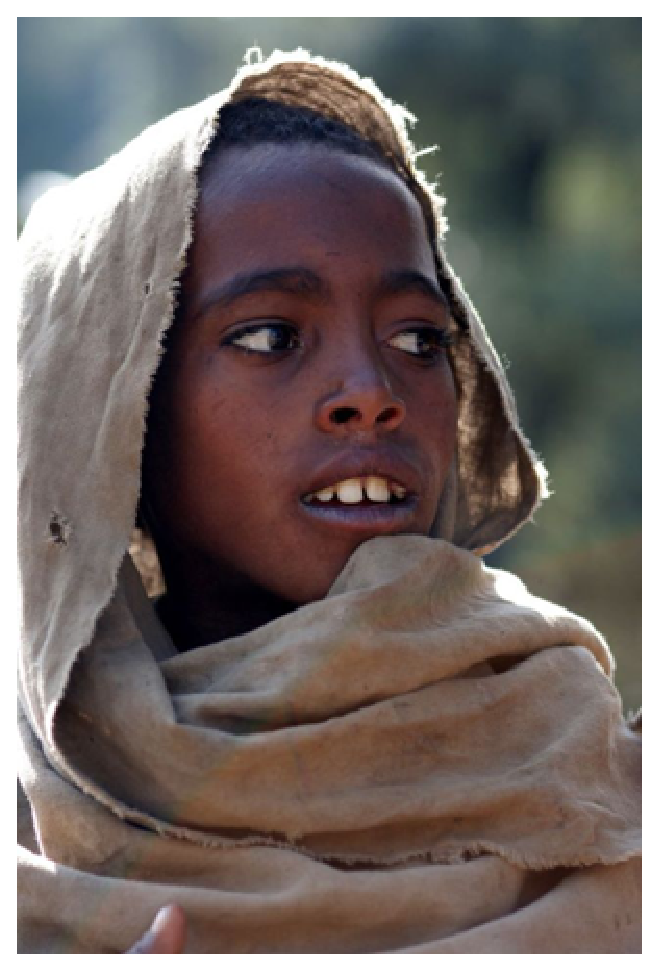
\includegraphics{etiopan.eps}}
    \reflectbox{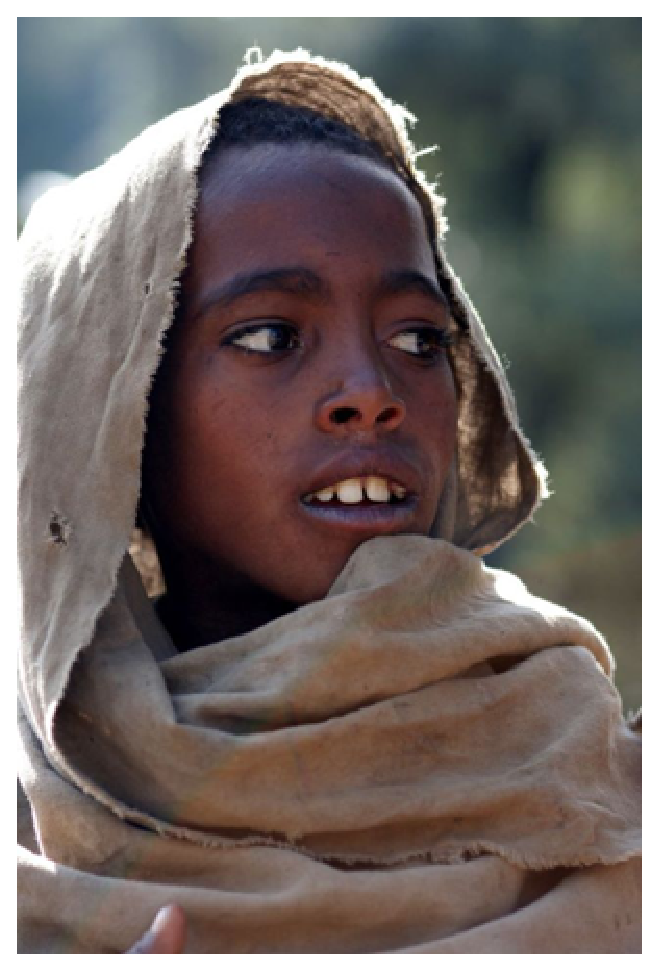
\includegraphics[scale=0.4]{etiopan.eps}}
    \caption{Malý Etiopánek a jeho bratříček}
    \label{etiopan}
\end{figure}


Rozdíl mezi vektorovým \dots

\begin{figure}[h]
    \scalebox{0.4}{
\includegraphics{oniisan.eps}}
    \centering
    \caption{Vektorový obrázek}
    \label{oniisan}
\end{figure}

\dots a bitmapovým obrázkem

\begin{figure}[h]
    \scalebox{0.6}{
\includegraphics{oniisan2.eps}}
    \centering
    \caption{Bitmapový obrázek}
    \label{oniisan2}
\end{figure}

\noindent
se projeví například při zvětšení. \par
Odkazy (nejen ty) na obrázky \ref{etiopan}, \ref{oniisan} a \ref{oniisan2}, na tabulky \ref{tab2_1} a \ref{tab2_2} a také na algoritmus \ref{FS} jsou udělány pomocí křížových odkazů. Pak je ovšem potřeba zdrojový soubor přeložit dvakrát. \par
Vektorové obrázky lze vytvořit i přímo v \LaTeX{u}, například pomocí prostředí \texttt{picture.}

\newpage

\begin{landscape}
    \begin{figure}[ht]
        \centering
        \setlength{\unitlength}{1mm}
        \resizebox{0.2\linewidth}{!}{
        \begin{picture}(200,400)
            \put(50,50){\line(1,0){200}}
            \put(50,50){\line(0,1){200}}
            \put(250,50){\line(0,1){200}}
    
            \put(50,250){\line(1,1){100}}
            \put(250,250){\line(-1,1){100}}
            \put(50,250){\line(1,0){200}}
    
            \put(150,50){\line(0,1){100}}
            \put(150,150){\line(1,0){50}}
            \put(200,50){\line(0,1){100}}
    
            \put(170,170){\line(1,0){30}}
            \put(170,170){\line(0,1){30}}
            \put(200,170){\line(0,1){30}}
            \put(170,200){\line(1,0){30}}
            
            \put(70,170){\line(1,0){30}}
            \put(70,170){\line(0,1){30}}
            \put(100,170){\line(0,1){30}}
            \put(70,200){\line(1,0){30}}
    
            \put(5,50){\line(0,1){100}}
            \put(10,150){\circle{80}}
            \put(0,190){\circle{30}}
            \put(20,190){\circle{30}}
            \put(10,220){\circle{20}}
    
            \put(300,400){\circle{80}}
            \put(300,480){\line(0,-1){60}}
            \put(300,320){\line(0,1){60}}
            \put(380,400){\line(-1,0){60}}
            \put(220,400){\line(1,0){60}}
        \end{picture}
        }
    \caption{Vektorový obrázek moderního bydlení vhodného pro 21. století. (Bud’to vytvořte stejný obrázek, anebo nakreslete pomocí picture váš vlastní domov.)}
    \end{figure}
\end{landscape}
\end{document}
